\section{流形假设与非线性降维}
\label{sec:13-Machine-Learning/04-Dimensionality-Reduction/04}

会议室的投影上是一张单细胞测序的二维图：两万个细胞、两万多个基因，压成平面上十几团彩色的点。有人指着图说，左上这团和右下那团离得最远，说明这两类细胞差异最大；中间那团面积最大，说明这个亚型数量最多。听起来都很合理。散会后你把 perplexity 从 30 改成 50 重跑一遍，团的相对位置换了，大小也变了，而数据一个字节没动。前三节的方法至少还给你一个可以对账的误差，这张图给的是什么？

\subsection{线性方法看不见弯曲的低维结构}

先说清楚为什么会走到非线性这一步。前三节把赌注押在同一种结构上：自由度集中在一个线性对象里——PCA 找方差最大的子空间，截断 SVD 找最佳低秩近似，矩阵补全假设背后是一张低秩表格。这个赌注常赢，但有一类情形它必输：低维结构确实存在，只是弯的。

标准玩具是瑞士卷。把一张二维薄片在三维里卷起来，

\[
\bigl(t\cos t,\ h,\ t\sin t\bigr),
\qquad
t\in\Bigl[\tfrac{3\pi}{2},\tfrac{9\pi}{2}\Bigr],\quad h\in[0,H],
\]

生成它的旋钮只有两个，观测坐标却是三个。麻烦不在于维数差，而在于没有任何二维平面能把它铺开：三个方向都有可观方差，斜着投影会把不同层折到一起，正对螺旋面投影则把高度压扁。

\begin{center}
\begin{tikzpicture}[>=stealth,scale=1.05]
\draw[black!35] plot[domain=270:810,samples=150]
  ({0.0027*\x*cos(\x)},{0.0027*\x*sin(\x)});
\draw[black,line width=1.4pt] plot[domain=450:810,samples=110]
  ({0.0027*\x*cos(\x)},{0.0027*\x*sin(\x)});
\fill[black] (0,1.215) circle (2.2pt);
\fill[black] (0,2.187) circle (2.2pt);
\node[font=\scriptsize,anchor=east,fill=white,inner sep=1pt] at (-0.1,1.215) {\(x_i\)};
\node[font=\scriptsize,anchor=east,fill=white,inner sep=1pt] at (-0.1,2.187) {\(x_j\)};
\draw[dashed,black] (0,1.215) -- (0,2.187);
\node[font=\scriptsize,anchor=west,fill=white,inner sep=1.5pt] at (0.12,1.70) {欧氏距离 \(\approx 2\pi\)};
\node[font=\scriptsize,anchor=west] at (1.05,-1.85) {沿曲面走完一整圈，弧长 \(\approx 2\pi t\)};
\draw[black,->] (1.0,-1.85) -- (0.35,-1.62);
\end{tikzpicture}
\end{center}

\emph{瑞士卷的横截面：两个点在三维空间里挨得很近，沿薄片走过去却隔着整整一圈。}

图里那对点解释了全部困难。参数相差 \(2\pi\) 的两个样本落在相邻两层，若高度相同，欧氏距离恰好是 \(2\pi\)，在三维里算得上近邻；沿薄片表面走过去要绕行一整圈，弧长约 \(2\pi t\)，随半径线性增长。欧氏几何说它们相邻，生成结构说它们隔着老远。任何以欧氏距离或线性投影为地基的方法，都会在这里把假邻居当成真邻居。

顺带把责任分清楚。PCA 并没有失职，它忠实完成了``最小平方重构''的承诺，只是这个承诺逐点计量误差，从不涉及点对之间的关系。方法做对了自己的题，题目本身换了。

\subsection{流形假设说的是自由度少，而且局部是平的}

瑞士卷是玩具，它背后的假设在真实数据里反复出现：高维观测往往集中在某个低维流形附近。理由有两条。

第一条来自生成机制。观测坐标多不等于自由度多。一张人脸照片有上百万像素，能自由变化的只有姿态、光照、表情那么几项；姿态角连续变化时像素值沿一条曲线走动，而这条曲线没有理由是直的。几十路传感器背后只有三五个物理状态，情形一样。

第二条解释了弯曲为什么仍然可处理：光滑流形在每一点附近都近似它的切空间。这正是\hyperref[sec:02-Calculus/06-Multivariable-Calculus/04]{``Jacobian 与多元链式法则''}里``可微即局部线性''的几何版本——生成映射 \(F\) 满足

\[
F(a+h)\approx F(a)+J_F(a)\,h ,
\]

尺度足够小时弯曲消失，邻域近似一个低维线性块。流形方法的全部工作原则由此而来：\textbf{信任小尺度上的线性，不信任大尺度上的线性}。

\subsection{保距路线：Isomap 把距离换掉}

既然问题出在欧氏距离，最直接的修法是换一把尺子。两点的``真实''距离应当沿流形表面量，也就是测地距离；图中那对点的测地距离是 \(2\pi t\) 而不是 \(2\pi\)。Isomap 分三步落实：每个点只与 \(k\) 个最近邻连边、边权取欧氏距离，因为短边落在切空间近似成立的尺度上；任意两点的测地距离用图上最短路径近似；最后把这个距离矩阵交给经典 MDS 求低维坐标。

第三步值得展开。给定平方距离矩阵 \(D=(d_{ij}^2)\)，双重居中

\[
B=-\tfrac12 JDJ,
\qquad
J = I-\tfrac1n\ind\,\ind^{\trans}
\]

把距离还原成内积矩阵，对 \(B\) 做特征分解取前几个特征对即得坐标。若输入距离本来就是欧氏的，经典 MDS 给出的正是 PCA 坐标，至多差一个正交变换。所以 Isomap 可以读作``先把尺子换对，再走第一节的老路''，新信息只在第二步进入：流形的拓扑通过邻接图参与了计算。

\subsection{保邻域路线：只承诺小尺度上的关系}

另一条路线更彻底。既然只有局部可信，那就只保局部，全局形状让它自己长出来。

LLE 分两步。先用每个点的近邻做线性重构，

\[
\min_{w}\ \sum_i\Bigl\|\,x_i-\sum_{j\in N(i)}w_{ij}x_j\Bigr\|^2,
\qquad \sum_{j\in N(i)}w_{ij}=1 ,
\]

权重 \(w_{ij}\) 刻画 \(x_i\) 周围的局部几何，且对旋转、平移、整体缩放不变。再固定权重不动，去找低维坐标让它们用同一组权重互相重构，

\[
\min_{Y}\ \sum_i\Bigl\|\,y_i-\sum_{j\in N(i)}w_{ij}y_j\Bigr\|^2 .
\]

局部结构被原样搬进低维空间，弯曲的全局形状在逐块粘贴中被展开。

t-SNE 走的是同一路线的概率版本：把高维的邻近关系写成一族概率 \(p_{ij}\)，在低维用重尾分布给出 \(q_{ij}\)，然后最小化 \(\KL(P\|Q)\)。UMAP 换了构图方式和损失细节，目标的性质是同一类。请注意目标函数里出现的量：全是邻居概率。\(\KL(P\|Q)\) 对``\(p_{ij}\) 大而 \(q_{ij}\) 小''惩罚很重——高维的邻居在低维必须还是邻居；反过来，``\(p_{ij}\) 小而 \(q_{ij}\) 大''几乎不受惩罚，本来离得远的点在图上放到哪里，目标函数并不在意。

\subsection{图上的簇间距离和簇大小都不可读}

上一段那句话是这一节最该被记住的东西，把它的后果说透。

\begin{center}
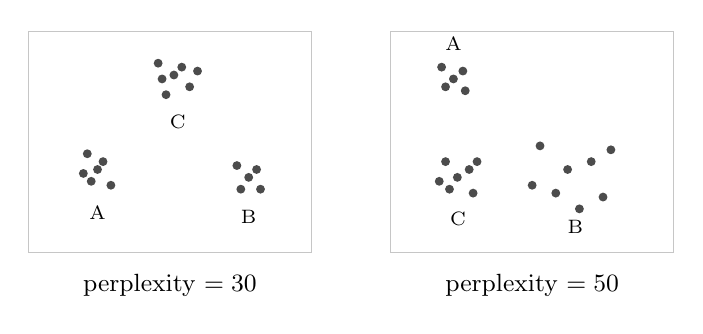
\begin{tikzpicture}[>=stealth,scale=1.0]
% 面板一
\draw[gray!45] (-0.2,-0.2) rectangle (3.4,2.6);
\foreach \c/\r in {0.6/0.7, 0.75/0.95, 0.55/1.05, 0.85/0.65, 0.68/0.85, 0.5/0.8}
  \fill[black!70] (\c,\r) circle (1.6pt);
\foreach \c/\r in {2.5/0.6, 2.7/0.85, 2.45/0.9, 2.75/0.6, 2.6/0.75}
  \fill[black!70] (\c,\r) circle (1.6pt);
\foreach \c/\r in {1.5/2.0, 1.75/2.15, 1.55/1.8, 1.85/1.9, 1.65/2.05, 1.95/2.1, 1.45/2.2}
  \fill[black!70] (\c,\r) circle (1.6pt);
\node[font=\scriptsize] at (0.68,0.3) {A};
\node[font=\scriptsize] at (2.6,0.25) {B};
\node[font=\scriptsize] at (1.7,1.45) {C};
\node[font=\small] at (1.6,-0.62) {perplexity \(=30\)};
% 面板二
\begin{scope}[shift={(4.6,0)}]
\draw[gray!45] (-0.2,-0.2) rectangle (3.4,2.6);
\foreach \c/\r in {1.9/0.55, 2.35/0.95, 1.7/1.15, 2.5/0.5, 2.05/0.85, 1.6/0.65, 2.6/1.1, 2.2/0.35}
  \fill[black!70] (\c,\r) circle (1.6pt);
\foreach \c/\r in {0.5/1.9, 0.72/2.1, 0.45/2.15, 0.75/1.85, 0.6/2.0}
  \fill[black!70] (\c,\r) circle (1.6pt);
\foreach \c/\r in {0.55/0.6, 0.8/0.85, 0.5/0.95, 0.85/0.55, 0.65/0.75, 0.9/0.95, 0.42/0.7}
  \fill[black!70] (\c,\r) circle (1.6pt);
\node[font=\scriptsize] at (2.15,0.12) {B};
\node[font=\scriptsize] at (0.6,2.45) {A};
\node[font=\scriptsize] at (0.66,0.22) {C};
\node[font=\small] at (1.6,-0.62) {perplexity \(=50\)};
\end{scope}
\end{tikzpicture}
\end{center}

\emph{同一批数据、同一个算法，只改一个超参数：三个簇还在，但谁挨着谁、哪个看起来更大，全变了。}

图上簇的相对位置没有含义，因为 \(\KL(P\|Q)\) 对远距离点对几乎不加约束；簇的面积也没有含义，因为局部尺度在优化中被自适应地拉伸——密集的簇会被撑开，稀疏的簇会被收拢，面积反映的是算法的带宽选择，不是样本量或方差。所以开头会议室里那两句话都不成立：``离得最远所以差异最大''不成立，``面积最大所以数量最多''也不成立。要回答这两个问题，得回到高维空间里去算——类间距离用原始特征或某个受控的度量算，样本量直接数。

图上唯一可信的是``哪些点反复地聚在一起''，而且这个结论也需要交叉检验：换随机种子、换 perplexity 或 \texttt{n\_neighbors}、换初始化，看簇的成员是否稳定。稳定的划分才值得进一步分析，随参数漂移的划分只是优化过程的痕迹。一个常被忽略的细节是初始化：用 PCA 前几维初始化通常比随机初始化更能保住一点全局结构，但那点全局结构是初始化带进来的，不是目标函数保证的。

\subsection{能力与脆弱来自同一个地方}

这些方法的力量与风险都长在邻接图上。近邻数 \(k\) 取小了，图断成互不连通的碎片，测地距离无从谈起；取大了，边直接跨过瑞士卷层与层之间的缝隙，最短路径被短路，测地距离退回欧氏距离，Isomap 悄悄退化成普通 MDS。层间的欧氏间隙只有约 \(2\pi\)，噪声稍大就会有样本被推到隔壁层附近，搭出本不该存在的桥——注意这种失败没有报错，算法照常输出一张漂亮的图。

还有一件工程上更要紧的事：Isomap、LLE、t-SNE 输出的是\emph{这批点}的坐标，不是一个能作用于新样本的函数。来了新数据，要么整个重跑，要么依赖额外的样本外扩展。相比之下 PCA 给出的 \(x\mapsto V_k^{\trans}(x-\bar x)\) 随时可用，可以原样封进推理流程。这是线性方法一个经常被低估的优点，也是为什么在生产系统里非线性降维多半只出现在探索阶段，而不出现在服务链路上。

两条线索到这里合流。前三节假设结构全局线性，换来显式映射、谱隙诊断和 Eckart--Young 那样的误差证书；本节假设结构只在局部线性，换来展开弯曲结构的能力，同时变得超参数敏感、噪声下脆弱、没有显式映射、也没有全局保证。选工具之前先问数据：有没有理由相信观测由远少于维数的旋钮经非线性映射生成？生成机制的知识、邻域关系在不同尺度下的稳定性，都算证据。若全局线性已经够用，不必为用不上的展开能力买下邻接图的脆弱性。

不过整个单元到此为止都在做同一个动作：把维数往下压。有些时候正确的动作恰好相反——把数据升到更高维反而让问题变简单。下一节处理这个看起来矛盾的方向。
